%%%%%%%%%%%%%%%%%%%%%%%%%%%%%%%%%%%%%%%%%%%%%%%%%%%%%%%%%%%%%%%%%%%%%%%%%%%%%%%%
%%%
%%% Dies ist unser Gemeinsames Skript zum Programmierpraktikum
%%% Shape Optimization with FEniCS im WS20/21
%%% Fügt gerne noch Pakete hinzu und definiert eure eigenen Befehle,
%%% das ganze sollte aber trotzdem übersichtlich und lesbar bleiben.



%%%%%%%%%%%%%%%%%%%%%%%%%%%%%%%%%%%%%%%%%%%%%%%%%%%%%%%%%%%%%%%%%%%%%%%%%%%%%%%%
%%%
%%% include packages and libraries
%%%
\documentclass[a4paper, 12pt]{scrartcl}
\usepackage{ngerman}
\usepackage[latin1]{inputenc}
\usepackage[T1]{fontenc}
\usepackage{ae,aecompl}
\usepackage{amsmath,amssymb,amstext}
\usepackage{listings}
\usepackage{graphicx}
\usepackage{tikz}
\usepackage{pgfplots}
\usetikzlibrary{patterns}
\usepackage{dsfont}
\usetikzlibrary{arrows,calc,shapes,decorations.pathreplacing}
\usepackage[automark]{scrpage2}

%%%%%%%%%%%%%%%%%%%%%%%%%%%%%%%%%%%%%%%%%%%%%%%%%%%%%%%%%%%%%%%%%%%%%%%%%%%%%%%%
%%%
%%% user defined commands
%%%

%%% \mygraphics{}{}{}
%% usage:   \mygraphics{width}{filename_without_extension}{caption}
%% example: \mygraphics{0.7\textwidth}{rolling_grandma}{This is my grandmother on inlinescates}
%% requires: package graphicx
%% provides: including centered pictures/graphics with a boldfaced caption below
%% 
\newcommand{\mygraphics}[3]{
  \begin{center}
    \includegraphics[width=#1, keepaspectratio=true]{#2} \\
    \textbf{#3}
  \end{center}
}
\newcommand{\R}{\mathbb{R}}
\newcommand{\dx}{\mathop{dx}}
\newcommand{\ds}{\mathop{ds}}
\newcommand{\Jhat}{\widehat{J}}
\DeclareMathOperator{\divergence}{div}
\tikzset{
	schraffiert/.style={pattern=north east lines,pattern color=#1},
	schraffiert/.default=black
}

%%%%%%%%%%%%%%%%%%%%%%%%%%%%%%%%%%%%%%%%%%%%%%%%%%%%%%%%%%%%%%%%%%%%%%%%%%%%%%%%
%%%
%%% define the titlepage
%%%

\subject{Shape optimization with FEniCS}
\titlehead{Programmier Praktikum WS2020/2021}

\title{Gemeinsame Dokumentation 
	\vspace{1cm}
	\mygraphics{0.7\textwidth}{graphics/shop1}{}
}
\author{Dozent: Dr. Martin Lenz}
\date{Bonn, am \today{}}

%%%%%%%%%%%%%%%%%%%%%%%%%%%%%%%%%%%%%%%%%%%%%%%%%%%%%%%%%%%%%%%%%%%%%%%%%%%%%%%%
%%%
%%% set heading and footer
%%%
\pagestyle{scrheadings}
\ifoot[]{Shape optimization with FEniCS - Gemeinsame Dokumentation}
\cfoot[]{}
\ofoot[]{\pagemark}

%%%%%%%%%%%%%%%%%%%%%%%%%%%%%%%%%%%%%%%%%%%%%%%%%%%%%%%%%%%%%%%%%%%%%%%%%%%%%%%%
%%%
%%% begin the document
%%%

\begin{document}

% \pagenumbering{roman} %% small roman page numbers

%%% include the title
% \thispagestyle{empty}  %% no header/footer (only) on this page
 \maketitle
%%% start a new page and display the table of contents
%\newpage
%\tableofcontents

 
\newpage


%%%%%%%%%%%%%%%%%%%%%%%%%%%%%%%%%%%%%%%%%%%%%%%%%%%%%%%%%%%%%%%%%%%%%%%%%%%%%%%%
%%%
%%% begin main document
%%% structure: \section \subsection \subsubsection \paragraph \subparagraph
%%%



%%%%%%%%%%%%%%%%%%%%%%%%%%%%%%%%%%%%%%%%%%%%%%%%%%%%%%%%%%%%%%%%%%%%%%%%%
%%% geschrieben von Jan Verhülsdonk:
\section{28.10.2020 - Einführung in die Form Optimierung}


\subsection{Linearisierte Elastizität}
Wir betrachten im Folgenden eine Deformation $\varphi: \Omega \subset \R^d \to \R^d$ und definieren die Verschiebung (engl. displacement) $u: \Omega \subset \R^d \to \R^d$ durch:
\[ \varphi(x)=x+u(x).\]

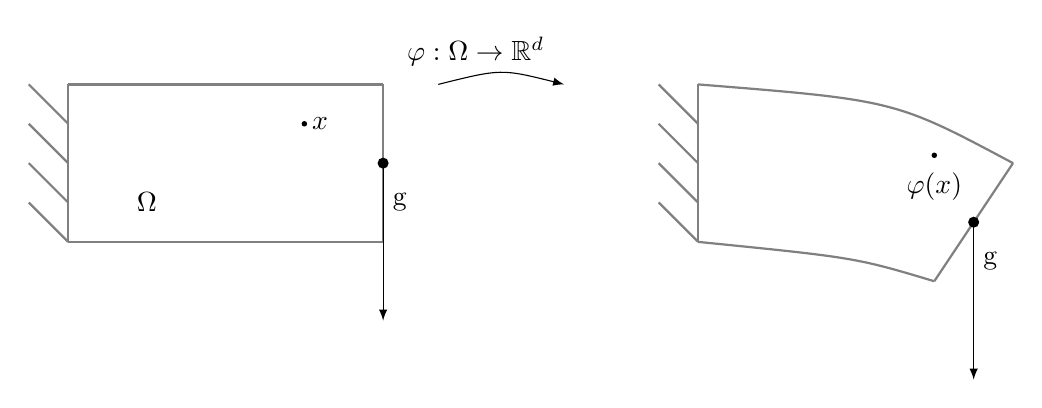
\begin{tikzpicture}
\draw[gray, thick] (0,2) -- (0,0);
\draw[gray, thick] (0,0) -- (4,0);
\draw[gray, thick] (4,0) -- (4,2);
\draw[gray, thick] (0,2) -- (4,2);
\draw[gray, thick] (0,1.5) -- (-0.5,2);
\draw[gray, thick] (0,1) -- (-0.5,1.5);
\draw[gray, thick] (0,0.5) -- (-0.5,1);
\draw[gray, thick] (0,0) -- (-0.5,0.5);
\draw[gray, thick] (8,2) -- (8,0);
\draw[gray, thick] (8,0) .. controls (10,-0.2) .. (11,-0.5);
\draw[gray, thick] (11,-0.5) -- (12,1);
\draw[gray, thick] (8,2) .. controls (10.5,1.8) .. (12,1);
\draw[gray, thick] (8,1.5) -- (7.5,2);
\draw[gray, thick] (8,1) -- (7.5,1.5);
\draw[gray, thick] (8,0.5) -- (7.5,1);
\draw[gray, thick] (8,0) -- (7.5,0.5);
\draw[->, >=latex] (4.7,2) .. controls (5.5,2.2) .. (6.3,2) node[above,near start] {$\varphi:\Omega \to \R^d$};
\fill (4,1) circle (2pt);
\draw[->, >=latex] (4,1) -- (4,-1) node[right,near start] {g};
\fill (11.5,0.25) circle (2pt);
\draw[->, >=latex] (11.5,0.25) -- (11.5,-1.75) node[right,near start] {g};

\draw(1,0.5) node {$\Omega$};
\fill (3,1.5) circle (1pt);
\draw(3.2,1.5) node {$x$};
\fill (11,1.1) circle (1pt);
\draw(11,0.7) node {$\varphi(x)$};
\end{tikzpicture}

Für kleine Verschiebungen lässt sich die Verzerrung (o.a. Dehnung, also lokale Längenänderungen) durch den linearisierten Dehnungstensor (strain tensor)
\[ \varepsilon (u) = \frac{ \nabla u + \nabla u^T }{2}\]
beschreiben. Die resultierende Spannung (stress) ist dann gegeben durch
\[ \sigma (u) = \lambda \divergence u \mathds{1}+ \mu \varepsilon(u).\]
$\lambda$ und $\mu$ sind materialabhängige Konstanten (Lamé-Parameter). Physikalische Deformationen minimieren dann Energien der Form:
\[ E(u) = \underbrace{\int_\Omega \sigma(u) : \varepsilon(u) \mathop{dx}}_{\text{gespeicherte Elastische Energie}} - \underbrace{ \int_{\partial \Omega} g \cdot u \mathop{ds}}_{\text{Nachgiebigkeit}}. \]
Die gespeicherte elastische Energie (stored elastic energy) ist bei kleinen Verschiebungen klein und wächst mit höheren Spannungen und Dehnungen. $g$ beschreibt am Rand wirkende äußere Kräfte. Die Nachgiebigkeit (compliance) wird klein, falls die Verschiebung sich an die Kräfte anpasst. Damit das für das Funktional ein Minimierer existeriert und man diesen berechnen kann, müssen in diesem Fall noch Dirichlet Randwerte ($u=0$ am linken Rand) gesetzt werden.

\subsection{Phasenfelder}
Um Formen und Geometrien mathematisch zu beschreiben gibt es mehrere Möglichkeiten. Wir werden zunächst sogenannte Phasenfelder (phase fields) benutzen. Das sind Funktionen $v: \Omega \to \R$ mit $v(x)\approx 1$ für den Teil von $\Omega$, der mit Material gefüllt ist und $v(x) \approx -1$ ansonsten. Dazwischen gibt es einen schmalen, glatten Übergang. \\

\vspace{0.5cm} 

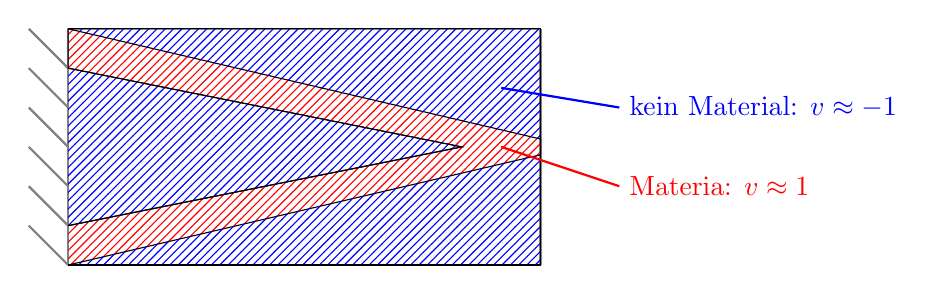
\begin{tikzpicture}
\draw[gray, thick] (0,3) -- (0,0);
\draw[gray, thick] (0,0) -- (6,0);
\draw[gray, thick] (6,0) -- (6,3);
\draw[gray, thick] (0,3) -- (6,3);
\draw[gray, thick] (0,2.5) -- (-0.5,3);
\draw[gray, thick] (0,2) -- (-0.5,2.5);
\draw[gray, thick] (0,1.5) -- (-0.5,2);
\draw[gray, thick] (0,1) -- (-0.5,1.5);
\draw[gray, thick] (0,0.5) -- (-0.5,1);
\draw[gray, thick] (0,0) -- (-0.5,0.5);
\draw[schraffiert=red] (0,0) -- (6,1.4) -- (6,1.6) -- (0,3) -- (0,2.5) -- (5,1.5) -- (0,0.5);
\draw[schraffiert=blue] (0,3) -- (6,3) -- (6,1.6);
\draw[schraffiert=blue] (0,0) -- (6,0) -- (6,1.4);
\draw[schraffiert=blue] (0,2.5) -- (5,1.5) -- (0,0.5);
\draw[red, thick] (5.5,1.5) -- (7,1) node[right]{Materia: $v\approx 1$};
\draw[blue, thick] (5.5,2.25) -- (7,2) node[right]{kein Material: $v\approx -1$};
\end{tikzpicture}

\vspace{0.75cm} 

Um diese Eigenschaften zu erzwingen, benutzt man ein double-well-potential (zu deutsch vielleicht zwei Mulden Potential) $\psi: \R \to \R$ mit $\psi(v)=\frac{9}{16}\left( v^2-1\right)^2$:

\vspace{0.5cm} 

\begin{tikzpicture}
\begin{axis}[
	domain=-1.5:1.5,
	xmin=-1.5, xmax=1.5,
	ymin=0, ymax=1,
	samples=400,
	axis y line=center,
	axis x line=middle,
	xlabel={$v$},
	ylabel={$\psi(v)$}
]
	\addplot+[mark=none] {(9./16.)*(x*x-1.)*(x*x-1.)};
\end{axis}
\end{tikzpicture}

\vspace{0.75cm} 


Zusammen mit einer entsprechenden charakteristischen Funktion $\chi:  \R \to \R$, $\chi(v)=\frac{1}{4}\left( v+1\right)^2$ lässt sich ein Strafterm $P(v)$ einführen
\[ P^\varepsilon(v)= \int_\Omega \alpha \underbrace{\frac{1}{2} \left( \varepsilon | \nabla v |^2 + \frac{1}{\varepsilon} \psi(v) \right)}_{\xrightarrow{\varepsilon \to 0} \text{Kantenlänge/Oberfläche}} + \underbrace{\beta \chi(v)}_{\text{Volumen}} \mathop{dx}  \]
der dafür sorgt, dass die Oberfläche und das Volumen der beschriebenen Form klein bleiben. $\alpha$ und $\beta$ sind hier Konstanten, die gewählt werden können, um den Oberflächenterm und den Volumenterm zu gewichten. \\
Für so beschriebene Flächen, lässt sich die gespeicherte elastische Energie für eine Verschiebung $u$ ausdrücken durch:
\[ E(u,v) = \int_\Omega ((1-\delta)\chi(v)+\delta) \sigma(u) : \varepsilon(u) \dx. \]
Für numerische Stabilität wählt man zumeist ein hard-soft-model, das heißt die Zwischenräume werden behandelt, als wären sie mit sehr weichem Material gefüllt. 

\subsection{Formoptimierung}
Je nachdem, welches Ziel die Formoptimierung haben soll, kann nun ein sogenanntes Kostenfunktional (cost functional) $J(u,v)$ aufgestellt werden. Soll die Form z.B. so gewählt werde, dass die Verformung unter einwirkenden Kräften minimal bleibt, wählt man:
\[ J(u,v) = P(v) + \int_{\partial \Omega} g \cdot u \ds \]
Hier muss darauf geachtet werden, dass $v(x)\approx1$, falls $g(x) \neq 0$ gilt. Das stellt sicher, dass an den Stellen wo Kräfte angreifen, Material vorhanden ist. Das Ziel der Formoptimierung ist nun:
\begin{align*}
	\text{Minimiere } J(u,v) \text{ bezüglich } v, \\
	\text{wobei} u \quad E(u,v) \text{ minimiert}
\end{align*}
Sei nun $u(v)$ der Minimierer von $E(\cdot,v)$ für festes $v$. Wir setzten nun
\[ \Jhat(v) = J(u(v),v). \]
Um die Ableitung von $\Jhat(v)$ nach $v$ zu berechnen, benutzen wir die Kettenregel und erhalten
\[ \Jhat_{,v}(v) =  J_{,u}(u(v),v)\underbrace{u_{,v}(v)}_{?} + J_{,v} (u(v),v) \]
Da die Abhängigkeit $u$ von $v$ nur über ein Minimierungsproblem gegeben ist, ist unklar, wie die Ableitung $u_{,v}(v)$ zu berechnen ist. Deshalb wählt man (wie bei anderen Optimierungsproblemen mit Nebenbedingungn) den Ansatz der Lagrangemultiplikatoren und setzen
\begin{align*}
L(u,v,p) = J(u,v) + E_{,u}(u,v)p.
\end{align*}
Notwendige Bedingungen zu Minimierung der Lagrange Funktion sind dann
\begin{align*}
(1)\quad \partial_p L &= E_{,u}(u,v)=0 &\text{-> das sichert unser Nebenbedingung} \\
(2)\quad \partial_u L &= J_{,u}(u,v) + E_{,uu} (u,v)p = 0 &\text{-> lineare Gleichung, definiert }p \\
(3)\quad\partial_v L &= \underbrace{J_{,v}(u,v) + e_{,uv}(u,v)p}_{= \Jhat_{,v} \text{ Form-Gradient, s.u.}} = 0
\end{align*}
Die dritte Gleichung liefert uns nach folgender Rechnung den Form-Gradienten:
\begin{align*}
\Jhat_{,v}(v) &= J_{,u}(u(v),v)u_{,v}(v) + J_{,v}(u(v),v) \\
&=-E_{,uu}(u(v),v)(p,u_{,v}(v)) + J_{,v}(u(v),v) \qquad \text{nach (2)} \\
&=-E_{,uu}(u(v),v)(u_{,v}(v),p) + J_{,v}(u(v),v) \qquad \text{mit Regularitätsannahmen} \\
&=E_{,uv}(u(v),v)p +J_{,v} (u(v),v)
\end{align*}
wobei der letzte Schritt aus Differentiation der notwendigen Bedingung nach $v$ folgt:
\begin{align*}
&E_{,u}(u(v),v) = 0\\
&\qquad \quad \downarrow \partial_v \\
E_{,uu}(u(v),v) &u_{,v}(v) + E_{,uv}(u(v),v) = 0
\end{align*}
Damit haben wir eine Darstellung des Formgradienten $\Jhat_{,v}$, die sich ohne $u_{,v}$ berechnen lässt.

\subsection{Was ist FEniCS?}
FEniCS ist eine Open-Source-Platform zur numerischen Lösung von Partiellen Differentialgleichungen mit Python. Wie Python ist FEniCS eine höhere Programmiersprache (also abstrakter und weniger Maschinennah als z.B. C) und erlaubt einen knappen und sehr natürlichen Programmierstil. FEniCS benutzt effiziente lineare Algebra Bibliotheken und erlaubt automatisierte Parallelisierung, ist also trotzdem recht effizient.

\subsection{Organisatorisches}
\begin{itemize}
	\item Die Programmierübungen dürfen in Gruppen mit bis zu 3 Studierenden abgeben werden
	\item Im Laufe des Praktikums wird dieses Latex-Dokument als gemeinsames Skript geführt und Inhalte, Präsentationen von Ergebnissen und Diskussionen des Praktikums festgehalten.
	\item für die Notenvergabe wird die \glqq Projektarbeit und Präsentation\grqq{} bewertet, also insbesondere:
	\begin{itemize}
		\item die Abgabe der Programmierübungen
		\item die Beteiligung in Diskussionen
		\item die Präsentation von Resultaten im Plenum (Jede Aufgabe wird von einer Gruppe vorgestellt)
		\item der Beitrag zum gemeinsamen Skript.
	\end{itemize} 
\end{itemize}

\subsection{Arbeitsumgebungen und erste Aufgabe}
\begin{itemize}
	\item FEniCS-Programme lassen sich in folgenden Arbeitsumgebungen ausführen:
	\begin{itemize}
		\item Anaconda (Python Distribution für wissenschaftliches Rechnen, kein FEniCS Paket für Windwos verfügbar)
		\item Docker (Software für Anwendungen in Containern)
		\item Ubuntu Pakete
	\end{itemize}
	\item Als Editor kann ein beliebiger Code Editor benutzt werden (z.B. Visual Studio Code)
	\item Zur Versionsverwaltung und zum Austausch von Code verwenden wir git (für die Abgabe der Übungsaufgaben GitHub Classroom)
	\item Zur Visualisierung von Resultaten eignet sich Paraview
\end{itemize}
Die ersten Aufgaben:
\begin{enumerate}
	\item Installieren Sie eine Arbeitsumgebung auf Ihrem PC.
	\item Führen Sie das Beispiel Programm von GitHub aus.
	\item Laden Sie ein ParaView Bild des Ergebnis auf GitHub hoch.
\end{enumerate}


%%%%%%%%%%%%%%%%%%%%%%%%%%%%%%%%%%%%%%%%%%%%%%%%%%%%%%%%%%%%%%%%%%%%%
%%% geschrieben von
%\section{04.11.2020 - ...}

%%%%%%%%%%%%%%%%%%%%%%%%%%%%%%%%%%%%%%%%%%%%%%%%%%%%%%%%%%%%%%%%%%%%%
%%% geschrieben von
%\section{11.11.2020 - ...}

%%%%%%%%%%%%%%%%%%%%%%%%%%%%%%%%%%%%%%%%%%%%%%%%%%%%%%%%%%%%%%%%%%%%%
%%% geschrieben von
%\section{18.11.2020 - ...}

%%%%%%%%%%%%%%%%%%%%%%%%%%%%%%%%%%%%%%%%%%%%%%%%%%%%%%%%%%%%%%%%%%%%%
%%% geschrieben von
%\section{25.11.2020 - ...}

%%%%%%%%%%%%%%%%%%%%%%%%%%%%%%%%%%%%%%%%%%%%%%%%%%%%%%%%%%%%%%%%%%%%%
%%% geschrieben von
%\section{02.12.2020 - ...}

%%%%%%%%%%%%%%%%%%%%%%%%%%%%%%%%%%%%%%%%%%%%%%%%%%%%%%%%%%%%%%%%%%%%%
%%% geschrieben von
%\section{09.12.2020 - ...}
% ...



\section{09.12.2020 Form Optimierung}
\subsection{Formulierung des Problems}

Die Formoptimierung ist ein Optimierungsproblem mit PDG als Nebenbedingungen.
Es hat die folgende Gestalt:

$$\mathrm{min}\ \  J(v, u)$$
$$s. t. \ \ \  ... \ \ \quad $$

Wobei $J(v, u)$ unsere Zielfunktion ist, die aus mehreren Termen besteht, $v$ ist ein Phasenfeld und $u$ 
die zugehoerige Loesung der linearen Elastizitaet bzw. minimiert die Elastische Energie. 
Ist die Loesung $u$ eindeutig, koennen wir $u$ als $u(v)$
ausdruecken und $J(v, u)$ auf eine Variable reduzieren: \\
$$\hat{J} (v) = J(v, u(v))$$
Man nennt $v$ auch Control/ Steuerungs Variable, $u$ den associated State, $\hat{J}$ das reduzierte Funktional und
das Problem allgemein Optimale Steuerung. \\  
Konkret haben wir (Vergleiche Kapitel 1): 

\[ E(u, v) = \underbrace{\int_\Omega \chi(v) (\sigma(u) : \varepsilon(u)) \mathop{dx}}_{\text{gespeicherte Elastische Energie}} - \underbrace{ \int_{\partial \Omega} g \cdot u \mathop{ds}}_{\text{Nachgiebigkeit}} \]

Statt nur der Charakterristischen Funktion, bedient man sich dem Hard-soft-approach. Dies hat den Vorteil, dass
$u$, wo kein Material ist, nicht beliebig ist:

\[ E(u,v) = \int_\Omega ((1-\delta)\chi(v)+\delta) \sigma(u) : \varepsilon(u) \dx\ + \ \int_{\partial \Omega} g \cdot u \mathop{ds}  \]

Ausserdem soll $v = 1$ auf $\Gamma \subseteq \partial \Omega$ und $g > 0$ auf $\Gamma$ sein. Nun kommen wir zum Ziel Funktional:
$$J(u, v) : = \int_{\partial \Omega} g \cdot u ds \ +\ \alpha \int_{\Omega} \frac{1}{2} (\epsilon |\nabla v|^2 + \frac{1}{\epsilon} 
\psi (v)) dx \ +\ \beta \int_{\Omega} \ \chi(v) dx$$

Insgesamt sieht unser Problem (P) wie folgt aus: 



\begin{tcolorbox}[ams gather]
\mathrm{min}_{u ,v}\ \ J(u, v) \qquad \qquad \qquad
 \\
\mathrm{s. t.}  \ \ u = min_{u'} E(u', v) \\
\ v \in V_{\mathrm{admissible}}
\end{tcolorbox}

\subsection{Lösen in Fenics}
\subsubsection{Dolfin-Adjoint}
Wir werden Dolfin-Adjoint (PyAdjoint) brauchen. Um dies zu installieren geht man wie folgt vor (http://www.dolfin-adjoint.org/en/latest/download/):
\begin{itemize}
	\item In Anaconda: conda install dolfin-adjoint
	\item In Docker: Image quay.io/dolfinadjoint/pyadjoint
	\item In Ubuntu: pip install git+https://github.com/dolfin-adjoint/pyadjoint.git@2019.1.0
\end{itemize}

Die Berechnung von $\hat{J}$ und $\partial_v \hat{J}$ läuft in Dolfin-Adjoint automatisch ab. Die Theorie dahinter findet man im Kapital 1. Dabei benutzt Dolfin-Adjoint das tape- und annotate feature. Diese zeichnen alle Rechnungen von Fenics auf, wobei die Gleichungen mit ihren Abhängigkeiten nochmal seperat abegspeichert werden, d. h. dass man im Programmablauf die Nebenbedingung einmal für irgendein beliebiges $v$ lösen muss. Danach liegt es auf dem Tape vor und kann abgerufen werden. Nun muss das Ziel Funktional mit den unabhängigen Variablen explizit angegeben werden. Danach werden $\hat{J}$ und $\partial_v \hat{J}$ automatisch berechnet.  \\ Dolfin-Adjoint bietet außerdem eine angepasste Version von scipy.minimize, welche Fenics Funktionen versteht. 


\subsubsection{Das Grundgerüst}
\begin{lstlisting}
from dolfin_adjoint import *
 
 mesh = ..
 V = ..
 u = Function(V) 
 ...
 E = ..
 J = ..
 solve(..E..)
 (Zusammenfügen der letzten beiden Übungen)

Jhat = ReducedFunctional(assemle(J), Control(v))
v = minimize(Jhat)
\end{lstlisting}


Die Funktion $\mathrm{minimize(Jhat)}$ hat einige Parameter. Darunter die Options, welche durch 
\begin{lstlisting}
options={'disp': True, 'ftol': 1e-8, 'gtol': 1e-8}
\end{lstlisting}
defniert werden. Die Option 'disp' besagt, ob nach jeder Iteration etwas zurück gegeben werden soll, 'ftol' ist die Toleranz in Bezug auf die Änderung des Funktionswertes und 'gtol' ist die Toleranz in Bezug auf die Norm des Gradienten (Abbruchkriterien). Desweiteren kann man durch method = '...' die Methode, die benutzt werden soll, angeben. Hier zum Beispiel:
\begin{itemize}
	\item Nelder-Mead
	\item L-BFGS-B \qquad      (Quasi-Newton-Verfahren kommt mit Bounds zurecht)
\end{itemize}
Als bounds werden auch Fenics Funktionen übergeben. Zum Beispiel:

\begin{lstlisting}
lb = project(Constant(-1000), V)
bc.apply(lb.vector())

ub = project(Constant(1000), V)
bc.apply(ub.vector())

v = minimize(Jhat, bounds=(lb, ub))
\end{lstlisting}


\subsubsection{Dolfin-Adjoint Taylor Test}
Zur Erinnerung: \\
Berechnung von $\hat{J}(v)$ die im Hintergrund passiert:
\begin{itemize}
	\item u(v) als Lösung von $\partial_u E(u, v) = 0$ für gegebenes $v$
	\item $\hat{J}(v) = J(v, u(v))$
\end{itemize}

"$\partial_v \hat{J}(v)$":
\begin{itemize}
	\item u(v) als Lösung von $\partial_u E(u, v) = 0$ für gegebenes $v$
	\item $\partial_u \partial_u E(u, v)(p) = \partial_u J(u, v) \qquad$ (p (Lagrange Multiplikator) wird berechnet, adjungierten Gleichung)
	\item $\partial_v \hat{J}(v) = $\partial_u \partial_v E(u(v), v)(p) + \partial_v J(v, u(v))$
\end{itemize}

Da das ganze im Hintergrund passiert, sollte man checken, ob die Ableitungen richtig berechnet werden, denn es kann zu Fehlern kommen. Nicht alle Konstrukte werden unterstützt z. B. Expression(...). Eine andere Fehlerquelle ist die Falscherkennung von Abhängigkeiten z. B. wenn Randwerte auf Knoten doppelt definiert werden (auch wenn sie gleich sind). Zum testen bietet Dolfin-Adjoint auch eine Funktion, die als Basis die Taylor Entwicklung verwenden: 
$$ \hat{J} (v + h \phi) =  \hat{J} (v) + \partial_v \hat{J} (v)(h \phi) + O(h^2)$$

\begin{lstlisting}
taylor_test(Jhat, v, phi)
oder wenn man einen linearen Abfall haben möchte:
taylor_test(Jhat, v, phi, dJdm = 0)
\end{lstlisting}
\subsubsection{Beispiel Szenarien}
Carrier Plate:
\begin{figure}[h]
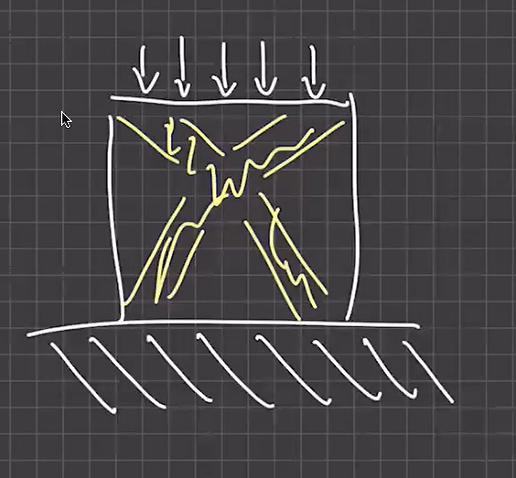
\includegraphics[width=8cm]{graphics/carrierplatepic2.png}
\end{figure}

Cantilever beam:
\begin{figure}[h]
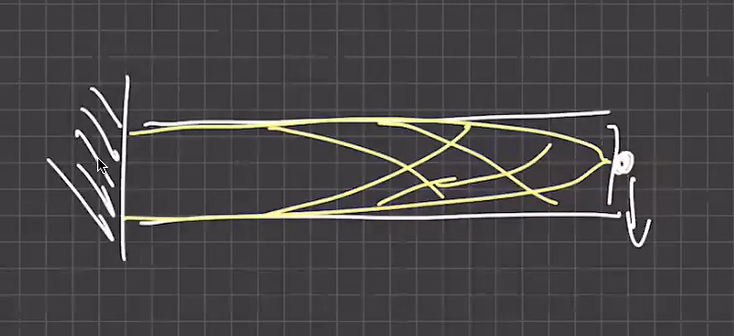
\includegraphics[width=8cm]{graphics/Cantipic.png}
\end{figure}

L-Shape:
\begin{figure}[h]
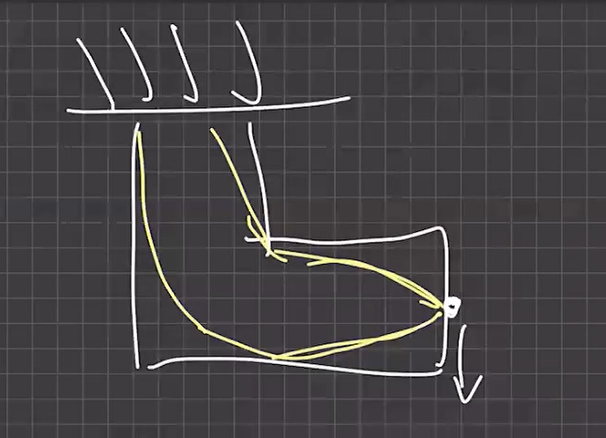
\includegraphics[width=8cm]{graphics/lshapepic.png}
\end{figure}





\end{document}
